\section{PHY Layer}
\label{sec:phy}

\subsection{Numerology}

The waveform is designed to pass through an ordinary SSB transceiver's
audio path (AGC off).  Table~\ref{tab:numerology} lists the parameters,
all taken from the article~\cite{habr_ofdm}.

\begin{table}[H]
    \centering
    \caption{OFDM numerology.}
    \label{tab:numerology}
    \small
    \begin{tabular}{@{}lp{8.5cm}@{}}
    \toprule
    \textbf{Parameter} & \textbf{Value} \\
    \midrule
    Sample rate       & 12\,kHz \\
    FFT size          & 128 bins $\rightarrow$ 93.75\,Hz subcarrier spacing \\
    Occupied band     & 300--2400\,Hz $\rightarrow$ bins 3--25, 23 subcarriers \\
    Pilots            & 7, Zadoff--Chu root 3, bins 3, 6, 10, 14, 17, 21, 25 \\
    Data carriers     & 16 \\
    Cyclic prefix     & 32 samples (25\,\%) \\
    Symbol tiling     & $4\times$ / $16\times$ / $64\times$ by link mode
                        (+6\,dB per $4\times$, coherent) \\
    CFO tolerance     & $\pm$375\,Hz design, $\pm$300\,Hz specified \\
    \bottomrule
    \end{tabular}
\end{table}

Symbol \emph{tiling} is the article's central trick for negative-SNR
operation: each OFDM symbol body is repeated back-to-back
\texttt{sym\_tile} times, and the receiver accumulates the repeats
coherently before the FFT.  Each $4\times$ factor buys $\approx$6\,dB
of effective SNR at a $4\times$ rate cost.

\subsection{Frame Structure}

Every frame (Figure~\ref{fig:frame_structure}) carries a two-stage
preamble --- Newman-phased tone combs~\cite{newman1965} for detection
and coarse CFO, then Zadoff--Chu symbols for sample-exact timing ---
followed by a header and the data block.  The header (25 bits:
\texttt{ver(2)\,|\,typ(3)\,|\,mod(2)\,|\,spd(2)\,|\,len(8)\,|\,CRC-8})
is always sent in the most robust configuration (BPSK, rate-1/3, six
tiled symbols = 93 coded bits); its \texttt{mod}/\texttt{spd}/%
\texttt{len} fields drive the data-block demodulation, and
\texttt{ver=2} marks an LDPC-coded data block
(Section~\ref{sec:coding}).  Preamble bins carry deliberate gain
($\times 2$ for ZC symbols, $\times\sqrt{5.75}$ for tone combs) so the
whole frame has uniform per-sample power --- Section~\ref{sec:sync}
shows why detection sensitivity depends on this.

\begin{figure}[H]
    \centering
    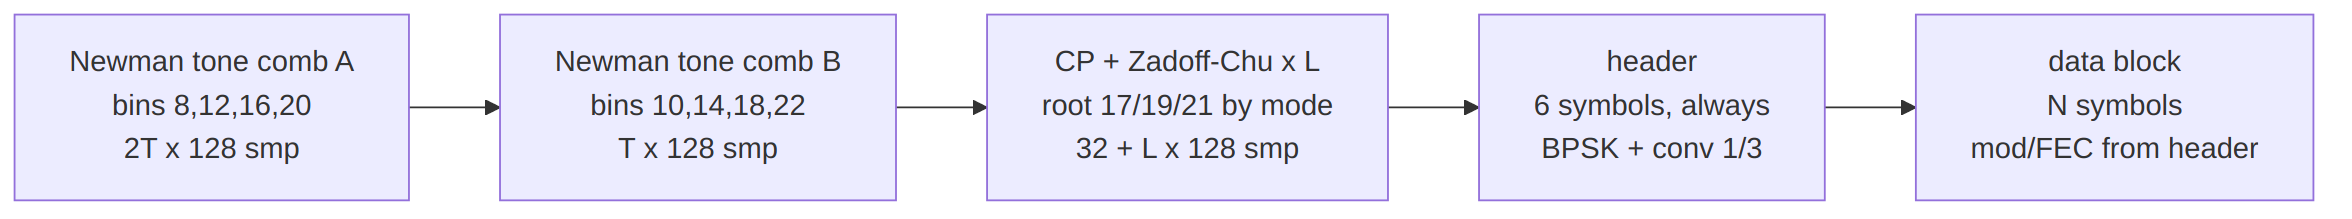
\includegraphics[width=\textwidth]{images/frame_structure.png}
    \caption{Frame structure.  $T$ is the mode's tone-tiling factor and
             $L$ the mode's Zadoff--Chu symbol count.}
    \label{fig:frame_structure}
\end{figure}

\subsection{Transmit Chain}

Figure~\ref{fig:tx_chain} shows the transmit chain
(\texttt{Transceiver.build\_frame}).  Packet bits (with CRC) are
FEC-encoded, zero-padded to a whole number of OFDM symbols
\emph{before} interleaving, interleaved over the 16 data carriers,
scrambled by a 15-bit LFSR, mapped (BPSK/QPSK/16-QAM Gray), and
assembled into OFDM symbols with the ZC pilots and a Hermitian mirror
so the time-domain signal is real.  After tiling and CP insertion the
preamble is prepended and a clip-and-filter stage (clip at
RMS+6\,dB, low-pass at 3\,kHz) bounds the PAPR.

\begin{figure}[H]
    \centering
    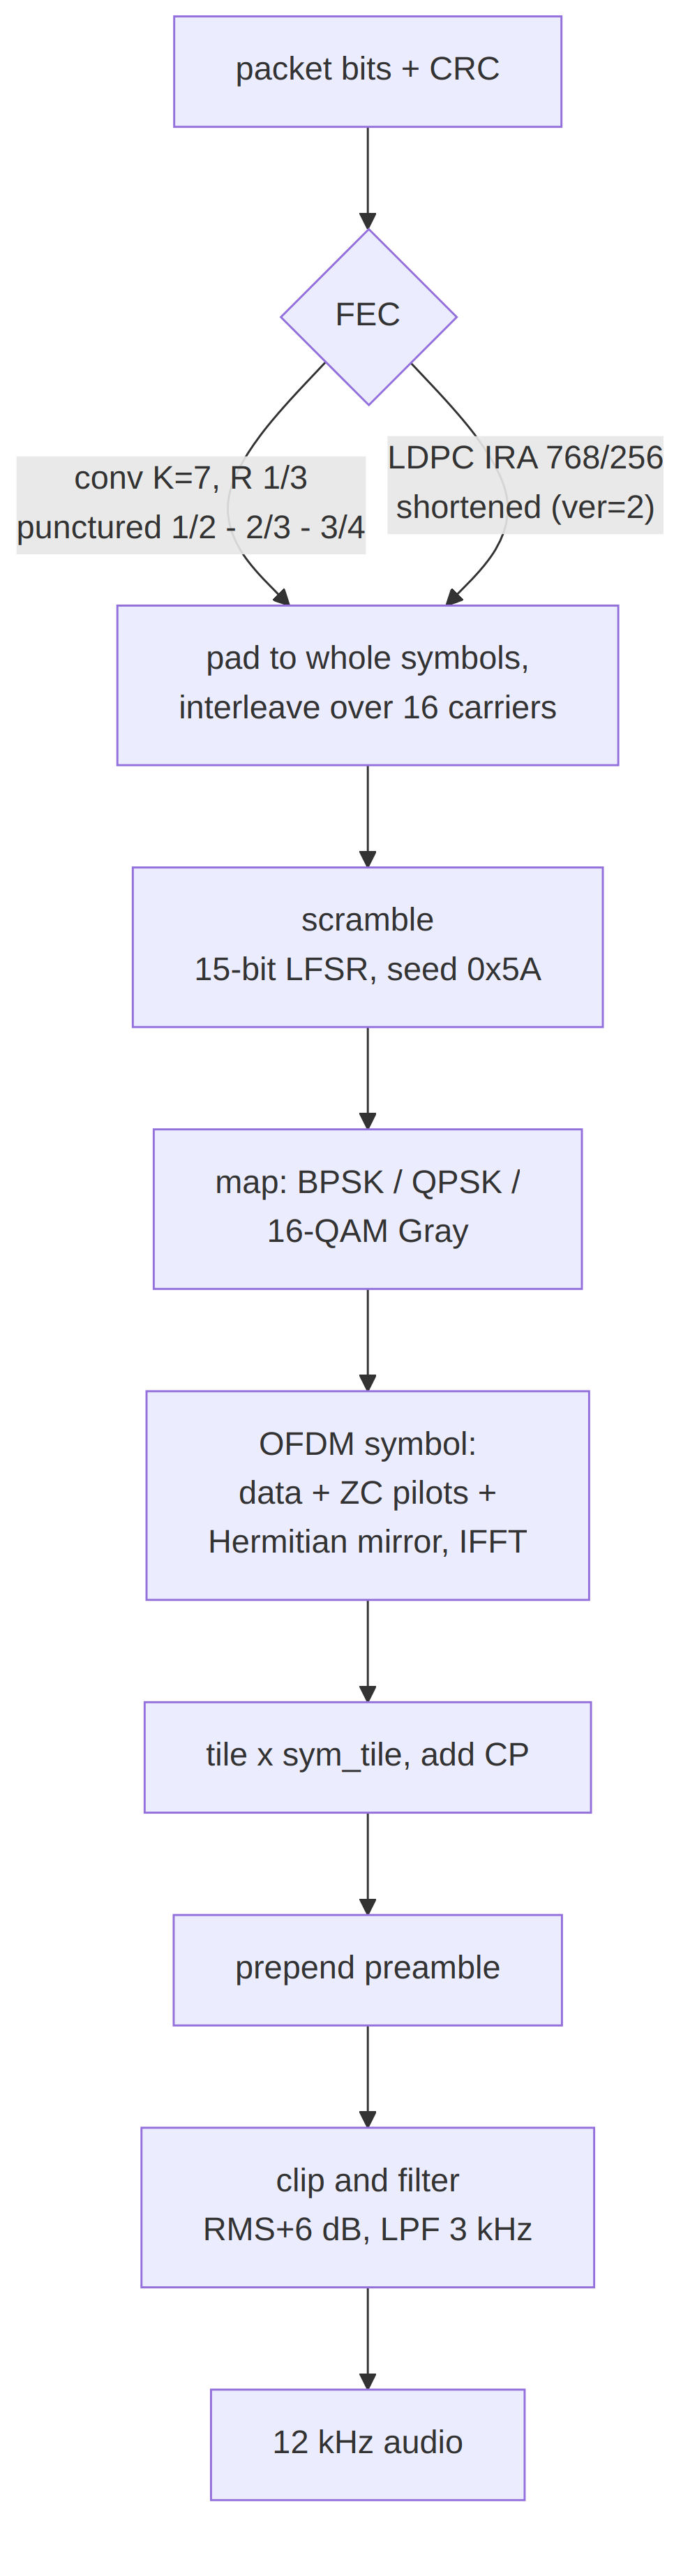
\includegraphics[width=0.62\textwidth,height=0.55\textheight,keepaspectratio]{images/tx_chain.png}
    \caption{Transmit chain.}
    \label{fig:tx_chain}
\end{figure}

Two ordering invariants are easy to break and worth stating: TX applies
interleave \emph{then} scramble, so RX must descramble \emph{then}
deinterleave; and because the FEC block is padded to whole symbols
before interleaving, RX must crop the deinterleaved stream back to the
codec's block length before decoding.

\subsection{Receive Chain}

Figure~\ref{fig:rx_chain} shows the receive chain
(\texttt{Transceiver.demod\_frame}).  After the analytic-signal
transform, synchronization runs in three stages (detailed in
Section~\ref{sec:sync}); the demodulator then processes each tiled
symbol: CP removal and coherent tile accumulation (with per-symbol
phase tracking), FFT, pilot-based channel estimation (zero-forcing
estimate at the pilots, Wiener smoothing with an exponential
frequency-correlation model of length 8 bins, MMSE equalization), and
LLR formation weighted by the per-carrier symbol SNR, clipped to
$\pm 20$.  One convention is load-bearing across four modules: LLR
sign is \textbf{positive = logical 1}, consistent with the article's
BPSK mapping table (the article's prose states the opposite of its own
code).

\begin{figure}[H]
    \centering
    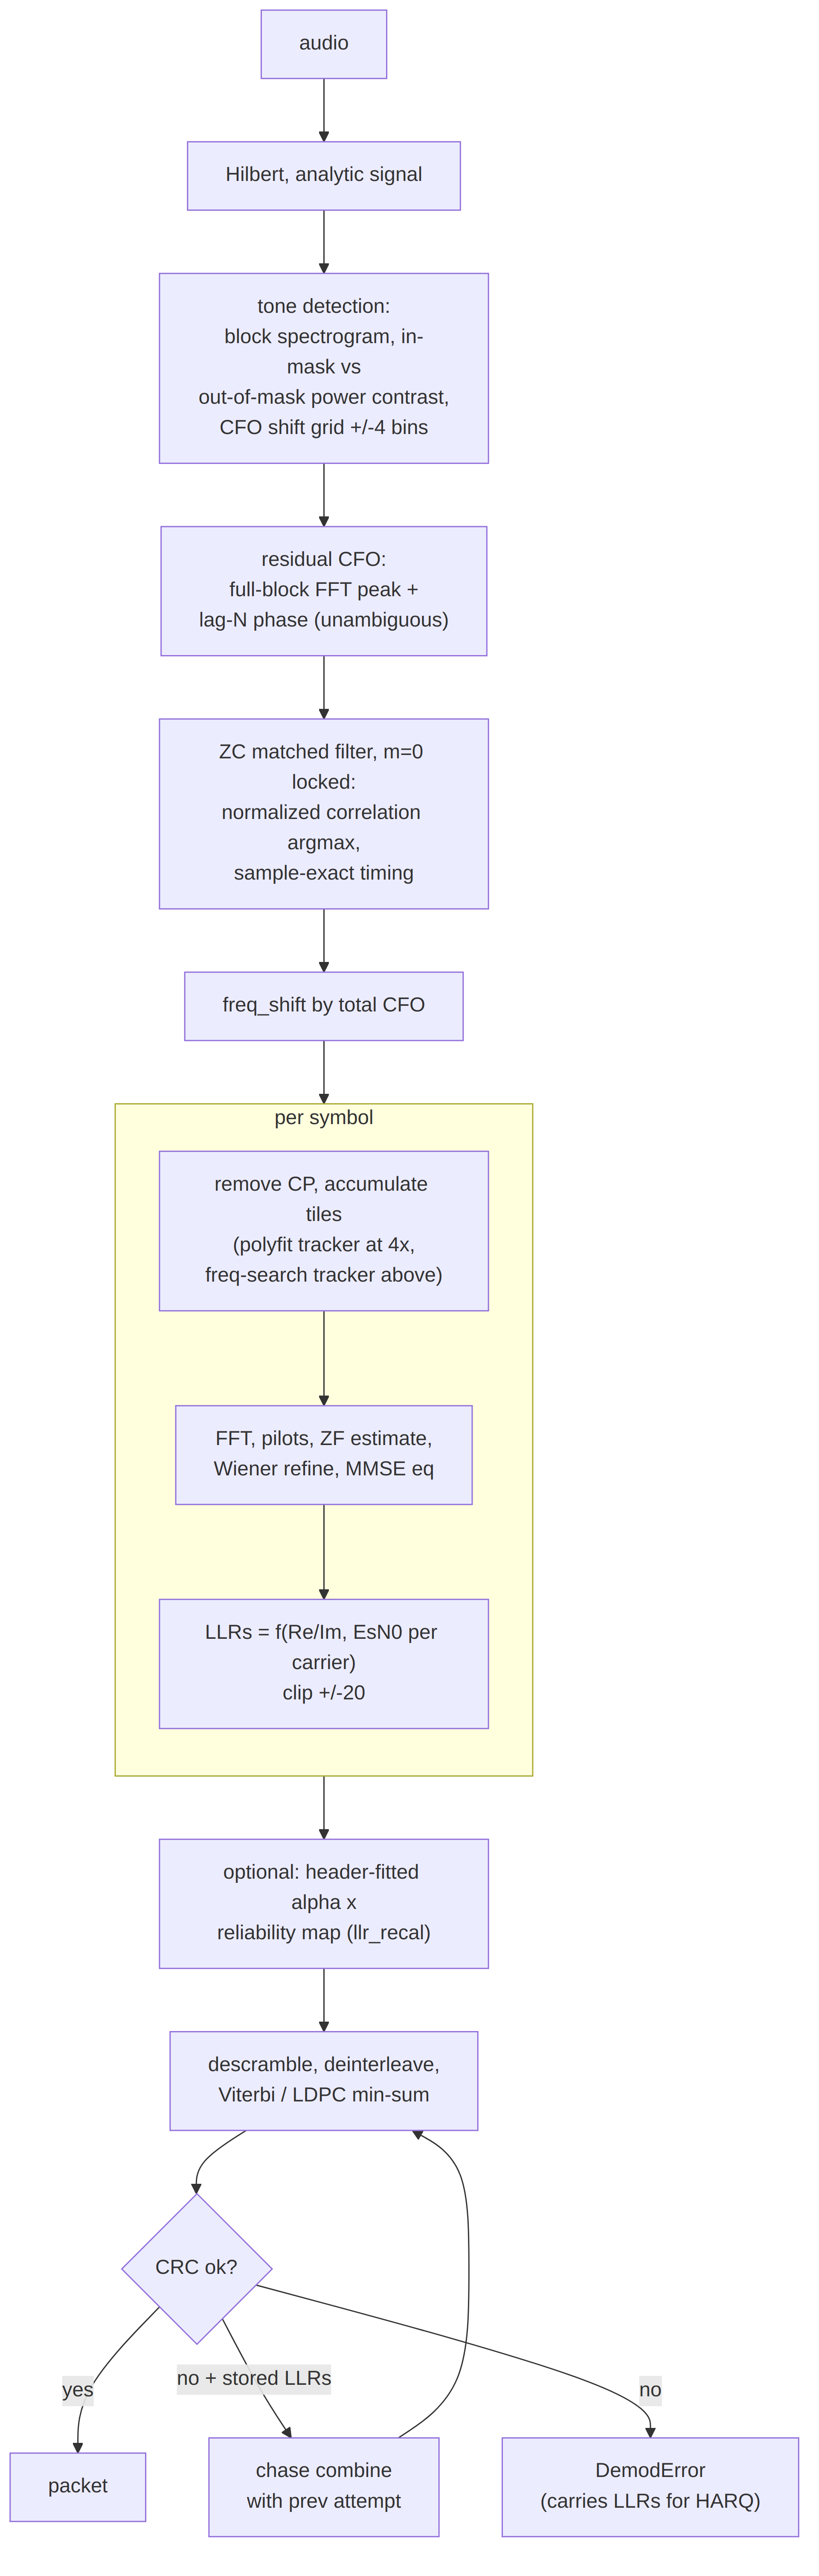
\includegraphics[width=0.72\textwidth,height=0.6\textheight,keepaspectratio]{images/rx_chain.png}
    \caption{Receive chain, including the opt-in recalibration stage
             (Section~\ref{sec:llr}) and the HARQ path
             (Section~\ref{sec:coding}).}
    \label{fig:rx_chain}
\end{figure}

A CRC failure does not simply discard the frame: the
\texttt{DemodError} exception carries the decoded header and the
data-block LLRs, which is what makes the chase-combining HARQ of
Section~\ref{sec:coding} possible without any extra signalling.

\subsection{Soft Demodulation: from Symbols to LLRs}
\label{sec:llr_math}

This subsection states exactly what the demodulator computes
(\texttt{OFDMModem.demodulate\_symbol\_cp\_soft}).  After tile
accumulation and FFT, each data carrier $k$ of a symbol obeys
\begin{equation}
    Y_k = H_k S_k + N_k,
    \qquad N_k \sim \mathcal{CN}(0, \sigma^2),
\end{equation}
where $H_k$ is the channel coefficient and $S_k$ the transmitted
constellation point.  With $\hat{H}_k$ the Wiener-smoothed pilot
estimate, the MMSE equalizer output is
\begin{equation}
    \hat{S}_k \;=\;
    \frac{Y_k\,\hat{H}_k^{*}}{|\hat{H}_k|^{2} + \hat{\sigma}^{2}} .
    \label{eq:mmse}
\end{equation}
The noise power $\hat\sigma^2$ is tracked decision-directed: the
mean-square error of $\hat S_k$ against the nearest constellation
point (per axis for BPSK/QPSK; against the sliced 16-QAM grid for
$\mu=4$), referred back through the channel by the mean
$|\hat H_k|^2$, and smoothed with an exponential filter
($\alpha = 0.1$) across symbols.  The per-carrier symbol SNR
\begin{equation}
    \rho_k \;=\; \frac{|\hat{H}_k|^{2}}{\hat{\sigma}^{2}}
\end{equation}
weights every LLR, so bits on faded carriers enter the decoder as
weak evidence rather than as confident errors.

The log-likelihood ratio of a bit $b$ is defined here as
\begin{equation}
    L(b) \;=\;
    \ln \frac{P(b = 1 \mid \hat{S})}{P(b = 0 \mid \hat{S})},
\end{equation}
i.e.\ \textbf{positive LLR means logical~1} --- the load-bearing sign
convention noted above.  Under the max-log approximation
$\ln \sum_i e^{x_i} \approx \max_i x_i$, the general form
\begin{equation}
    L(b_i) \;\approx\; \rho_k
    \Bigl( \min_{s \in \mathcal{S}_0^{(i)}} |\hat{S}_k - s|^2
         - \min_{s \in \mathcal{S}_1^{(i)}} |\hat{S}_k - s|^2 \Bigr)
\end{equation}
collapses to closed forms per modulation (as implemented; overall
scale is immaterial to the scale-invariant Viterbi and min-sum
decoders, but the \emph{shape} across carriers and bit positions is
what Section~\ref{sec:llr} calibrates):
\begin{align}
    \text{BPSK:}\quad
        & L = 4\,\rho_k \operatorname{Re}\hat{S}_k, \\
    \text{QPSK:}\quad
        & L_I = 2\,\rho_k \operatorname{Re}\hat{S}_k,
    \qquad L_Q = 2\,\rho_k \operatorname{Im}\hat{S}_k, \\
    \text{16-QAM (Gray, unit } a = g/\sqrt{10}\text{):}\quad
        & L_{b_0} = 2\,\rho_k \operatorname{Re}\hat{S}_k / g,
    \qquad L_{b_1} = 2\,\rho_k
        \bigl(2a - |\operatorname{Re}\hat{S}_k|\bigr) / g,
    \label{eq:qam_llr}
\end{align}
with the imaginary-axis pair $L_{b_2}, L_{b_3}$ analogous, and $g$ the
per-symbol gain estimate.  The 16-QAM forms are the piecewise-linear
max-log metrics of the Gray mapping: the outer bit ($b_0$) is the axis
sign, the inner bit ($b_1$) discriminates inner from outer amplitude
levels, changing sign at $|\!\operatorname{Re}\hat S| = 2a$.  All LLRs
are clipped to $\pm 20$ before decoding.
